% !TeX spellcheck = it_IT
\newpage
\section{Principi di progettazione}
Le tecniche di progettazione e le good practice mirano a produrre un sistema che realizzi \textbf{requisiti funzionali} e di \textbf{qualità}, mantenendolo facilmente \textbf{manutenibile} e \textbf{riusabile}.
\subsection{Principi generali}
\subsubsection{Information hiding}
Consiste nella separazione tra l'\textbf{interfaccia} visibile e il \textbf{corpo}, ovvero l'implementazione che è privata e/o nascosta. I componenti o i moduli sono come \textbf{black box} che forniscono e richiedono funzionalità. Rendono nota all'esterno solo la loro \textbf{interfaccia} ma nascondono algoritmi e strutture dati usati internamente.\\
I vantaggi principali sono:
\begin{itemize}
	\item \textbf{Comprensibilità}: non servono i dettagli implementativi per usare una feature
	\item \textbf{Manutenibilità}: si può cambiare il corpo di un'unità senza cambiarne altre
	\item \textbf{Team work}: corpi di unità diverse possono essere sviluppate da team indipendenti
	\item \textbf{Sicurezza}: i dati di un'unità sono modificabili solo internamente
\end{itemize}

\begin{observation}[Incapsulamento]
	L'incapsulamento è diverso dall'information hiding: il primo rappresenta la capacità degli oggetti di mantenere al loro interno attributi e metodi ed è una proprietà dei linguaggi di programmazione. Permette, \textit{senza garantire}, l'information hiding tramite i costrutti \textit{public} e \textit{private}
\end{observation}

Lo standard de-facto per l'accesso agli attributi privati, che quindi ne nasconde la rappresentazione, è tramite un'interfaccia di getter e setter:
\begin{itemize}
	\item \textbf{getter}: restituisce un attributo come valore e senza cambiare lo stato dell'oggetto
	\item \textbf{setter}: modifica lo stato dell'oggetto cambiando il valore dell'attributo
\end{itemize}

\subsubsection{Astrazione}
Il principio di astrazione si applica a:
\begin{itemize}
	\item \textbf{Controllo}: una procedura è vista come modulo di astrazione del flusso di controllo, nascondendo l'algoritmo utilizzato. Sono organizzate in classi di moduli e costituiscono la libreria.
	\item \textbf{Dati}: la struttura dati, che regolamenta accesso e modifica, è astratta, garantendo un'interfaccia stabile indipendentemente dal cambio di implementazione. Non sono puramente funzionali in quanto le operazioni offerte possono cambiare lo stato.
\end{itemize}

\subsubsection{Coesione}
La coesione è quanto strettamente correlate sono le funzionalità offerte da un modulo o da una componente. Funzionalità vicine devono stare nella stessa unità e un sistema è coeso se tutti gli elementi di ogni unità sono strettamente collegati. Esistono diversi tipi di coesione:
\begin{itemize}
	\item \textbf{Funzionale}: gli elementi collaborano per realizzare una funzionalità
	\item \textbf{Temporale}: gli elementi sono azioni che devono essere eseguite in uno stesso arco di tempo (difficilmente coese e riutilizzabili)
	\item \textbf{Logica}: gli elementi sono correlati logicamente ma non funzionalmente (e.g. raccolta dati, analisi e generazione dei report). Possono essere operazioni correlate ma funzioni significativamente diverse o operazioni debolmente connesse e difficilmente riutilizzabili
	\item \textbf{Accidentale}: gli elementi non sono correlati ma sono piazzati assieme
\end{itemize}

\subsubsection{Disaccoppiamento}
Indica quanto sono slegate le unità di progettazione in termini di dipendenze funzionali o messaggi. In un sistema molto accoppiato (\textbf{high coupling}) le modifiche alle varie unità impattano anche le altre a distanza, rendendo difficile la manutenzione. In quelli poco accoppiati (\textbf{low coupling}) l'impatto delle modifiche è limitato.

\begin{observation}
	Un alto grado di coesione contribuisce a ridurre il grado di accoppiamento.
\end{observation}

\subsection{Collezione di principi}
\subsubsection{SOLID}
SOLID include cinque principi di base per progettazione e sviluppo object oriented.
\begin{wrapfigure}[5]{r}{3.5cm}
	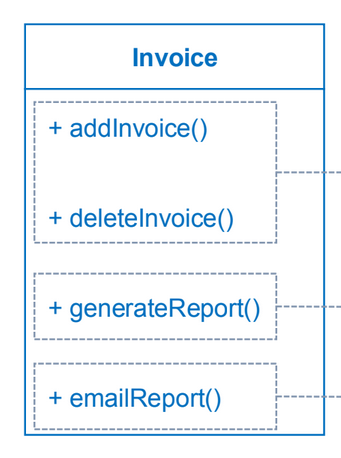
\includegraphics[width=3.5cm]{singleresp}
\end{wrapfigure}
\paragraph{Single Responsibility} Una classe o metodo deve avere un solo motivo per cambiare: un cambiamento deve impattare solo la classe che realizza quella funzionalità, se ci sono più motivi vanno create più classi. Deve quindi essere \textbf{funzionalmente coesa}.\\
Le eccezioni a questa regola sono:
\begin{itemize}
	\item La separazione di una classe introdurrebbe complessità non necessaria
	\item Un motivo di cambiamento è tale se è una reale possibilità di \\cambiamento nel sistema
\end{itemize}

\paragraph{Open Closed} Le entità software devono essere aperte per estensione ma chiuse per modifiche. Se i requisiti cambiano si deve estendere il comportamento aggiungendo nuovo codice, senza cambiare quello esistente e funzionante. Si può implementare tramite classi \textbf{astratte} e \textbf{concrete}, \textbf{delega} e \textbf{plugin}.

\paragraph{Liskov Substitution}
Deriva dal principio di sostituzione di Barbara Liskov.
\begin{definition}[Principio di sostituzione]
	Dato $S$ \textbf{sottotipo} di $T$, $o_s$ e $o_t$ oggetti di tipo rispettivamente $S$ e $T$ e $P$ un programma definito in termini di $T$. Se $o_s$ è usato al posto di $o_t$, il comportamento di $P$ è immutato. 
\end{definition}
\begin{center}
	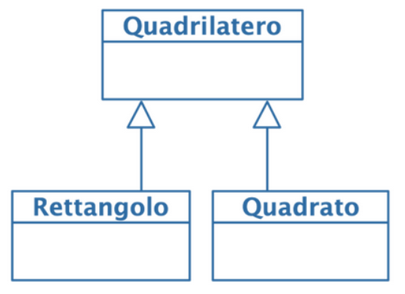
\includegraphics[scale=.4]{subst}
\end{center}

\paragraph{Interface Segregation} Le interfacce devono essere a \textbf{grana fine} e \textbf{specifiche} per ogni cliente: i client non devono dipendere da interfacce che non usano e si devono mettere solo i metodi utilizzati.
\begin{example}
	Ad esempio un lavoratore lavora e mangia. Può essere umano o robot ma quest'ultimo non può mangiare. Conviene quindi separare l'interfaccia del lavoratore da quello del mangiatore e il robot implementerà solo la prima.
\end{example}

\paragraph{Dependency Inversion} Si deve programmare per l'interfaccia e non per l'implementazione: i moduli di alto livello non devono dipendere da quelli di basso livello ma devono entrambi dipendere da \textbf{astrazioni} che a loro volta non devono dipendere dai dettagli.

\begin{example}
	Dati dei moduli per leggere, scrivere e copiare, è necessario che questi non dipendano, ad esempio, dal mezzo su cui eseguire le operazioni. Potrebbero essere implementate per la lettura da tastiera e scrittura su schermo oppure lettura da tastiera e scrittura su disco.
\end{example}

\subparagraph{Dependency Injection} È una forma di inversione delle dipendenze dove il cliente non sa come costruire i servizi che vuole chiamare ma delega ad un \textbf{iniettore}, che poi a sua volta passa al client i servizi. È quindi sufficiente sapere solo le interfacce dei servizi che definiscono come il client può usarli e in questo modo le responsabilità di costruzione e di utilizzo sono separate.

\subsubsection{GRASP}
Questa famiglia di principi di progettazione si compone di: \textbf{General Responsibility Assignment Software Patterns}. La progettazione è guidata dai \textbf{casi d'uso} che vengono realizzati in termini di oggetti collaborativi utilizzando diagrammi e pattern e assegnando responsabilità alle classi.\\

In particolare le \textbf{responsabilità} sono obblighi che un oggetto ha, definiti in termini di comportamento, e legate al dominio del problema. Possono essere di due tipi:
\begin{itemize}
	\item \textbf{Fare}: fare qualcosa (e.g. creare un oggetto o fare un calcolo) o iniziare, controllare e coordinare le azioni di altri oggetti
	\item \textbf{Conoscere}: conoscere i dati privati, gli oggetti correlati, i dati che possono derivare o calcolare. Generalmente si deducono dal modello di dominio.
\end{itemize}

\begin{observation}
	Una responsabilità non è un metodo: questi ultimi sono implementati per soddisfare le prime e la traduzione da responsabilità a metodi dipende dalla \textbf{granularità} della prima.
\end{observation}

\subsection{Delega}
L'ereditarietà presenta alcuni problemi: obbliga ad ereditare tutti i metodi anche se non rilevanti o non adatti e rende la sottoclasse strettamente legata all'implementazione della superclasse. La delega, al contrario, rende esplicito l'utilizzo parziale e consente di \textbf{controllare quanti e quali} metodi la classe delegata usa. Il costo è rappresentato dai metodi di delega aggiuntivi.\\

La delega riduce leggermente le \textbf{prestazioni} per l'invocazione di un altro oggetto rispetto all'uso di un metodo ereditato. Inoltre non può essere usata con classi astratte e non impone una struttura al progetto.

\subsection{Qualità del software}
\subsubsection{Functional suitability}
Il grado con cui un prodotto o un sistema fornisce funzionalità che soddisfino le richieste esplicite ed implicite quanto usato sotto certe condizioni. Si divide in:
\begin{itemize}
	\item \textbf{Functional completeness}: quando le funzionalità offerte coprono i task specificati e gli obiettivi degli utenti considerati
	\item \textbf{Functional correctness}: quanto siano accurati i risultati forniti agli utenti considerati
	\item \textbf{Functional appropriatness}: quanto le funzionalità offerte facilitano il raggiungimento del task e gli obiettivi considerati
\end{itemize}

\subsubsection{Performance efficiency}
Il grado con cui un sistema esegue le sue funzioni nella quantità di tempo specificata e con determinati parametri di output assieme alla sua efficienza nell'uso delle risorse date determinate condizioni. Si divide in:
\begin{itemize}
	\item \textbf{Time behaviour}: quanto vengono rispettati i requisiti in termine di \textit{response time} e \textit{throughput}
	\item \textbf{Resource utilization}: quanto vengono rispettati i requisiti  in termini di \textit{quantità} e \textit{tipologia} di risorse computazionali utilizzate
	\item \textbf{Capacity}: quanto vengono rispettati i requisiti in termini di capacità (limiti massimi)
\end{itemize}

\subsubsection{Compatibility}
Il grado con cui un sistema scambia informazioni con altri ed esegue funzioni mentre condivide lo stesso ambiente comune e le stesse risorse. Si divide in:
\begin{itemize}
	\item \textbf{Co-existance}: quanto il sistema rimane efficiente mentre condivide ambiente e risorse
	\item \textbf{Interoperability}: quanto il sistema riesce a scambiare informazioni con altri e sfruttare quelle ricevute
\end{itemize}

\subsubsection{Interaction capability}
Il grado con cui un sistema può interagire con utenti specifici per scambiare informazioni nell'interfaccia utente per completare task in diversi contesti. Si divide in:
\begin{itemize}
	\item \textbf{Appropriatness recognizability}: quanto gli utenti riconoscono se il sistema è appropriato
	\item \textbf{Learnability}: quanto le funzionalità sono apprendibili da un utente in un certo lasso di tempo
	\item \textbf{Operability}: quanto sia facile operare e controllare il sistema
	\item \textbf{User error protection}: quanto il sistema prevenga errori operativi
	\item \textbf{User engagement}: quanto \textit{engaging} sia il sistema
	\item \textbf{Inclusivity}: quanto il sistema può essere utilizzato da utenti con background diversi
	\item \textbf{User assistance}: quanto il sistema può essere usato da utenti diversi per gli stessi task
	\item \textbf{Self-descriptiveness}: quanto bene sono presentate le informazioni e le funzionalità per rendere ovvio l'utilizzo del sistema
\end{itemize}

\subsubsection{Reliability}
Il grado con cui un sistema esegua determinate funzioni in determinate condizioni per un certo periodo di tempo. Si divide in:
\begin{itemize}
	\item \textbf{Faultlessness}: quanto il sistema funziona senza fallimenti
	\item \textbf{Availability}: quanto il sistema sia operativo ed accessibile quando richiesto
	\item \textbf{Fault tolerance}: quanto il sistema riesca a ripristinare lo stato desiderato in caso di fallimento
\end{itemize}

\subsubsection{Security}
Il grado con cui un sistema riesce a difendersi da attacchi e proteggere le informazioni e i dati. Si divide in:
\begin{itemize}
	\item \textbf{Confidentiality}: quanto il sistema assicura che i dati siano accessibili solo a persone autorizzate
	\item \textbf{Integrity}: quanto il sistema assicura che lo stato del sistema e i dati siano protetti da modifiche non autorizzate
	\item \textbf{Non-repudiation}: quanto sia dimostrabile che azioni ed eventi abbiano avuto luogo
	\item \textbf{Accountability}: quanto sono tracciabili le azioni di una entità
	\item \textbf{Authenticity}: quanto è dimostrabile che l'identità di un soggetto o risorsa sia effettivamente quella
	\item \textbf{Resistance}: quanto il sistema è resistente da attacchi di malintenzionati
\end{itemize}

\subsubsection{Maintainability}
Il grado di efficacia ed efficienza con cui un sistema può essere modificato per migliorarlo, correggerlo o adattarlo a cambi dell'ambiente e dei requisiti. Si divide in:
\begin{itemize}
	\item \textbf{Modularity}: quanto poco i cambiamenti di un modulo di un sistema impattano sugli altri
	\item \textbf{Reusability}: quanto è riusabile il sistema e le sue parti
	\item \textbf{Analyzabilty}: quanto è facile analizzare l'impatto di un eventuale cambiamento, diagnosticare le cause di eventuali problemi o identificare le parti da modificare
	\item \textbf{Modifiability}: quanto sia modificabile il sistema senza degradarne le qualità
	\item \textbf{Testability}: quanto sia facile determinare i criteri di test e testare effettivamente il sistema
\end{itemize}

\subsubsection{Flexibility}
Il grado con cui un prodotto può essere adattato ai cambiamenti dei requisiti, del contesto o dell'ambiente.
\begin{itemize}
	\item \textbf{Adaptability}: quanto il sistema è adattabile a cambiamenti HW e SW degli ambienti di esecuzione
	\item \textbf{Scalability}: quanto bene il sistema gestisce i cambiamenti di workload e variability
	\item \textbf{Installability}: quanto efficientemente il sistema può essere installato o disinstallato
	\item \textbf{Replaceability}: quanto il sistema può sostituirne un altro sviluppato per gli stessi scopi
\end{itemize}

\subsubsection{Safety}
Il grado con cui un prodotto evita stati in cui la vita umana, la salute o gli oggetti siano messi in pericolo.
\begin{itemize}
	\item \textbf{Operational constraint}: quanto il sistema è vincolato a rimanere nei parametri di sicurezza
	\item \textbf{Risk identification}: quanto eventuali rischi di sicurezza sono identificati
	\item \textbf{Fail safe}: quanto in caso di fallimenti o pericoli il sistema riesca ad agire in safe mode
	\item \textbf{Hazard warning}: quanto il sistema fornisca avvisi su rischi inaccettabili per gli operatori in modo che essi possano reagire spontaneamente
	\item \textbf{Safe integration}: quanto il sistema riesca a mantenere la \textit{safety} se integrato con altri sistemi
\end{itemize}

\newpage
\subsection{Qualità delle implementazioni}
\subsubsection{Client-Server 2-N tier}
\begin{table}[!h]
	\centering
	\begin{tabular}{|c|p{10cm}|}
		\hline
		\textbf{Disponibilità} & I server di ogni tier possono essere replicati quindi in caso di fallimento il problema sarebbe minimo.\\
		\hline
		\textbf{Fault tolerance}&Se un client sta comunicando con un server che fallisce, la richiesta viene reindirizzata ad un server replicato in maniera trasparente. \\
		\hline
		\textbf{Modificabilità} & Il disaccoppiamento e la coesione di questa architettura favoriscono la modificabilità.\\
		\hline
		\textbf{Performance} & Buone performance ma bisogna tenere d'occhio il numero di threads, la velocità delle comunicazioni e il volume dei dati scambiato.\\
		\hline
		\textbf{Scalabilità} & Basta replicare i server di ogni tier. Unico bottleneck potrebbe essere la base di dati in comune.\\
		\hline
	\end{tabular}
\end{table}

\subsubsection{Pipes and filters}
\begin{table}[!h]
	\centering
	\begin{tabular}{|c|p{10cm}|}
		\hline
		\textbf{Disponibilità} & Avendo componenti e possibilità di connetterli sufficienti a formare una catena.\\
		\hline
		\textbf{Fault tolerance}&Occorre riparare una catena interrotta usando componenti replica. \\
		\hline
		\textbf{Modificabilità} & Presente se le modifiche interessano una o poche componenti.\\
		\hline
		\textbf{Performance} & Dipende dalla capacità del canale di comunicazione e dalla performance del filtro più lento.\\
		\hline
		\textbf{Scalabilità} & Ok.\\
		\hline
	\end{tabular}
\end{table}

\subsubsection{Publish-Subscribe}
\begin{table}[!h]
	\centering
	\begin{tabular}{|c|p{10cm}|}
		\hline
		\textbf{Disponibilità} & Si possono creare cluster di dispatcher.\\
		\hline
		\textbf{Fault tolerance}&Si crea un dispatcher replica. \\
		\hline
		\textbf{Modificabilità} & Si possono aggiungere publisher e subscriber ponendo attenzione al formato dei messaggi.\\
		\hline
		\textbf{Performance} & Ok ma con un compromesso tra velocità e requisiti tipo affidabilità e/o sicurezza.\\
		\hline
		\textbf{Scalabilità} & Con un cluster si può gestire un volume molto elevato di messaggi.\\
		\hline
	\end{tabular}
\end{table}

\subsubsection{P2P}
\begin{table}[!h]
	\centering
	\begin{tabular}{|c|p{10cm}|}
		\hline
		\textbf{Disponibilità} & Dipende dal numero di nodi, si assume di si.\\
		\hline
		\textbf{Fault tolerance}&Gratis. \\
		\hline
		\textbf{Modificabilità} & Si se si è interessati solo alla parte di comunicazione.\\
		\hline
		\textbf{Performance} & Dipende dal numero di nodi, dalla rete e dagli algoritmi.\\
		\hline
		\textbf{Scalabilità} & Gratis.\\
		\hline
	\end{tabular}
\end{table}